% !TEX root = WWW.tex
\begin{figure*}[!ht]
\centering
\hspace*{-1em}
\subfloat[\small \textsc{google}]{
    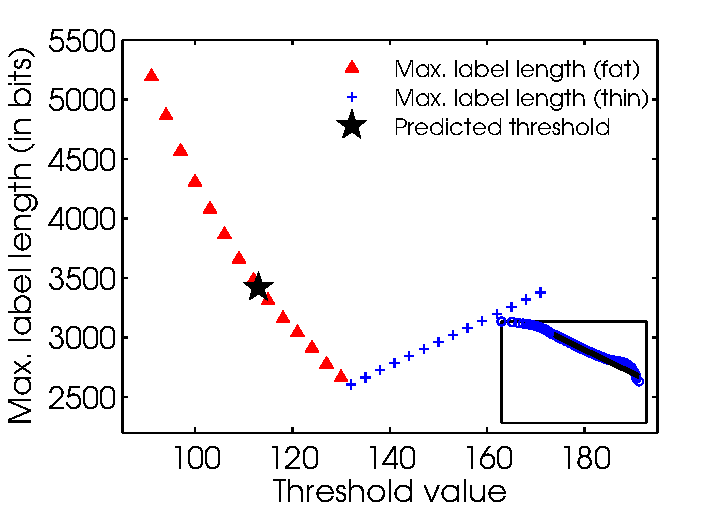
\includegraphics[width=0.45\textwidth]{Figures/web-google-revised.pdf}
}\hspace*{-1.9em}
\subfloat[\small \textsc{youtube}]{
    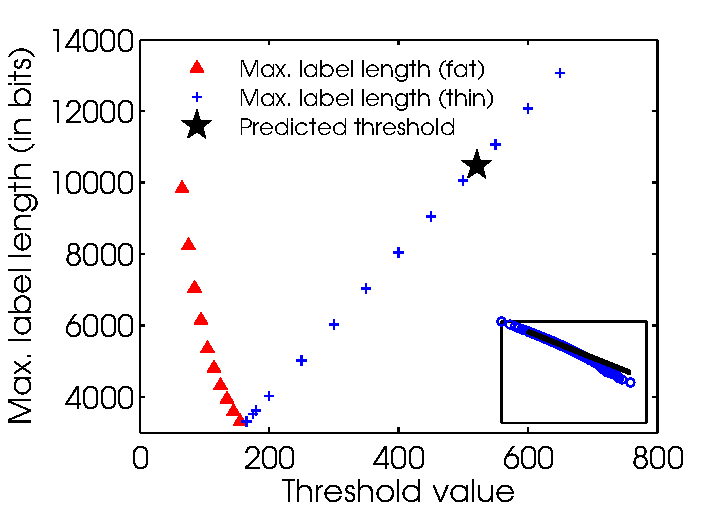
\includegraphics[width=0.45\textwidth]{Figures/web-youtube-revised.pdf}
}%
\hfill
\subfloat[\small \textsc{wikitalk}]{
    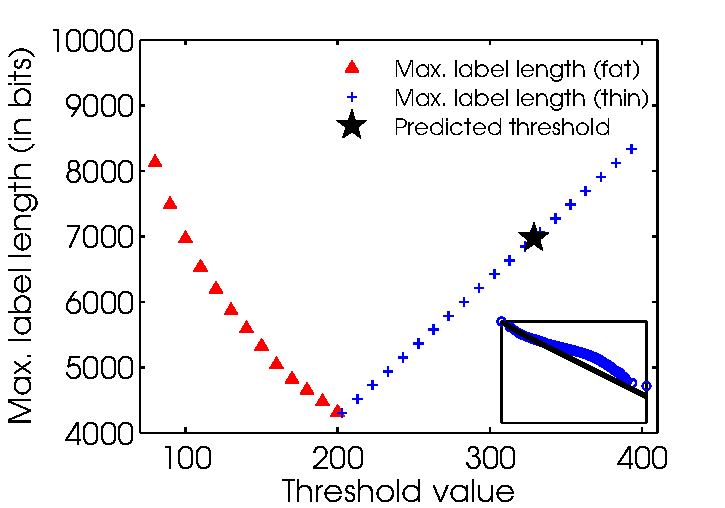
\includegraphics[width=0.45\textwidth]{Figures/web-wikitalk-revised.pdf}
}\hspace*{-1.9em}
\subfloat[\small \textsc{livejournal}]{
    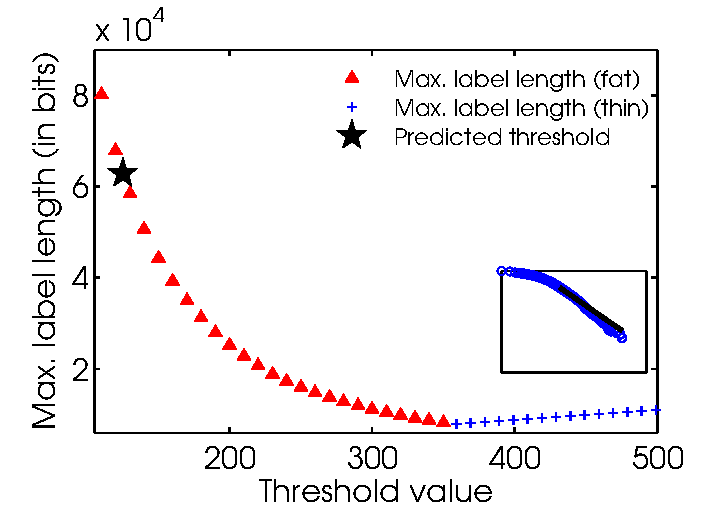
\includegraphics[width=0.45\textwidth]{Figures/web-livejournal-revised.pdf}
}%
\caption{Predicted and empirical thresholds for the \textsc{google}, \textsc{youtube}, \textsc{wikitalk} and \textsc{livejournal} datasets. The inset show the MLE fitted power law, using the method of Clauset et al.\ \cite{clauset2009power}, where data points are blue circles and the power law is shown as a black solid. The exponents of the power laws are shown in Table \ref{t:datasets}.}%
\label{f:bla2}%
\end{figure*}